\documentclass[main.tex]{subfiles}

\begin{document}


\vspace{3mm}

\section{Introduction}

\subsection{Applications of dynamical systems}

\hrulefill

Jan 25, 2017

\begin{itemize}
    \item
    Hoop with a sliding bead (see fig \ref{fig:hoop-and-bead})

    Small $\omega \implies \phi = 0\deg$

    Large $\omega \implies \phi = 90\deg$

    Goal: Find critical value $\omega$ so that the bead begins to move.
        \begin{figure}[ht]
        \centering
        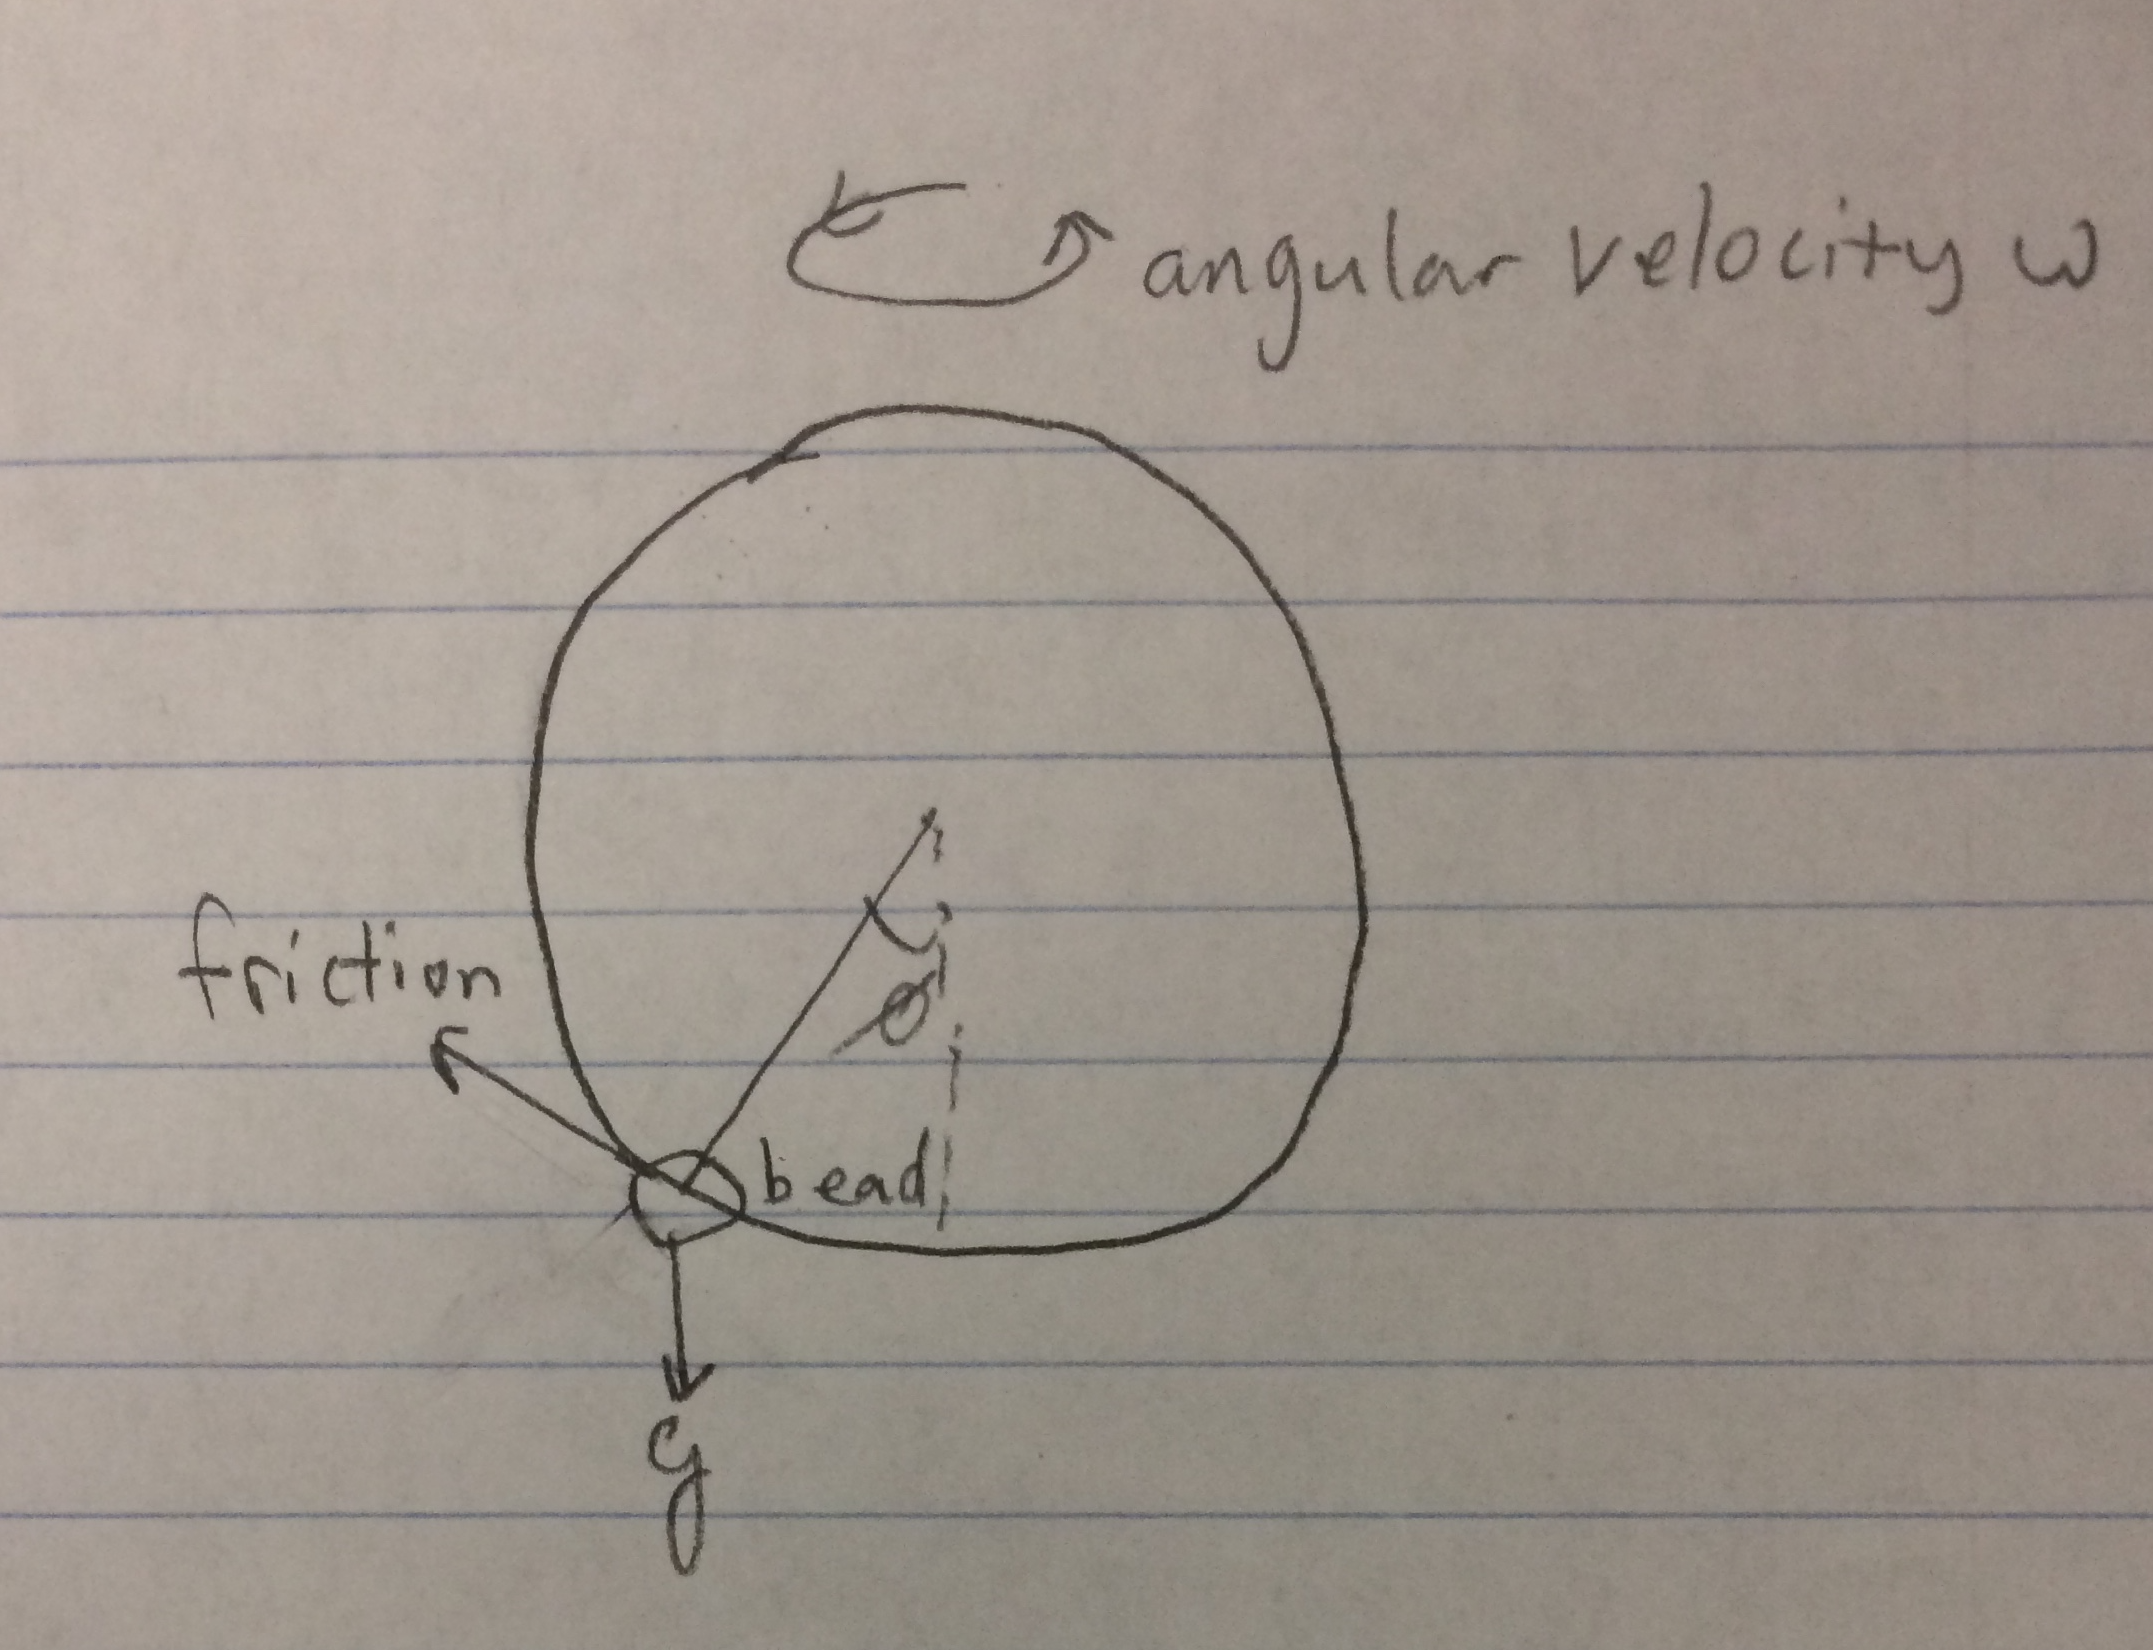
\includegraphics[width=0.5\textwidth]{hoop-fig}
        \caption{A hoop is rotated about it's axis with angular velocity $\omega$.}
        \label{fig:hoop-and-bead}
        \end{figure}
    \item
    Tipping points (insect outbreaks, climate change modeling) $\implies \textrm{ bifurcation theory}$

    Help to understand when and how the dynamics change, and the results.

    \item
    Temporal oscillations
    \[\left.
    \begin{array}{lr}
        \text{Circadion Rhythms (biological cycle).} \\
        \text{Cell cycles.}
    \end{array}\right\} \implies\textrm{ Identify and construct periodic solutions of models.}\]
    \item
    Spatial Structures (phase transitions, see fig \ref{fig:phase-transition}).
        \begin{figure}[ht]
        \centering
        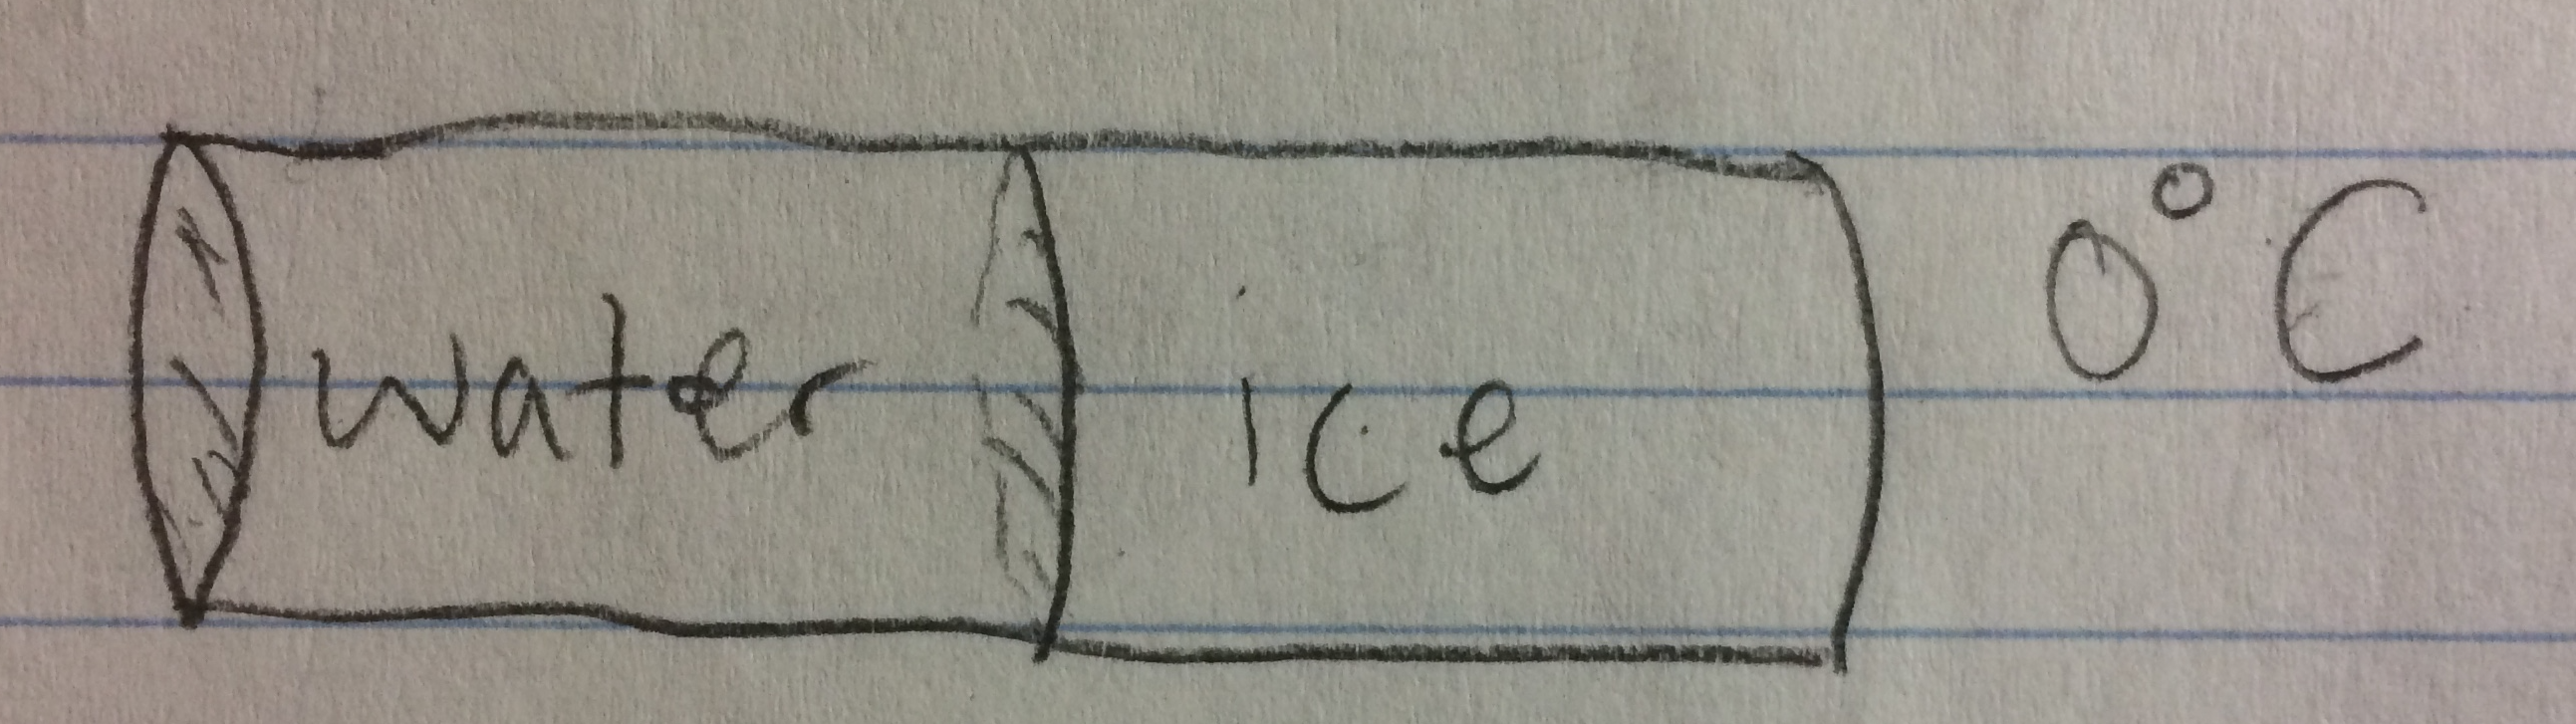
\includegraphics[width=0.5\textwidth]{phase-transition}
        \caption{A cylinder filled half with ice and half with water. The goal of dynamical systems is to find the evolution of the interfact between the water and ice as temperature, time, and the spatial coordinate changes.}
\label{fig:phase-transition}
\end{figure}
\end{itemize}

\subsection{Applications of chaotic dynamics}
\begin{itemize}
    \item \textbf{Double Pendulum}

    Dynamics are complicated, unpredictable and very sensitive to initial conditions

    Goal: Classify, predict, and quantify behaviours

    \item \textbf{Lorenz System (1963)}

    \begin{equation*}
    \label{eq:Lorenz-System}
        \begin{cases}
            \dot{x} &= \sigma(x-y) \\
            \dot{y} &= rx - y - xz \\
            \dot{z} &= xy - bz
        \end{cases}
    \end{equation*}

    Parameters: $\sigma, r, b$

    Variables: $x, y, z$

\end{itemize}

\subsection{Math Content}
\[
\begin{array}{lr}
    \textrm{Bifurcation theory} & \textrm{How changes effect solutions} \\
    \textrm{Existence and Uniqueness Theorem} & \textrm{Proof} \\
    \textrm{Dynamical systems analysis} & \textrm{Periodic, invariant \& homoclinic orbits; index theory} \\
    \textrm{Chaotic dynamics} & \textrm{Predict dynamics; noninteger dimensions} \end{array}\]

\end{document}
